\documentclass[acmsmall,screen,review,anonymous]{acmart}
\usepackage{amsmath,amsfonts,amsthm}
\let\Bbbk\relax
\usepackage{amssymb}
\usepackage{algorithm}
\usepackage{algorithmic}
\usepackage{graphicx}
\usepackage{siunitx}
\usepackage{booktabs}
\usepackage{multirow}
\usepackage{url}
\graphicspath{{./figures/}}
\newtheorem{theorem}{Theorem}
\newtheorem{corollary}[theorem]{Corollary}
\newtheorem{proposition}[theorem]{Proposition}
\newtheorem{lemma}[theorem]{Lemma}
\newtheorem{definition}{Definition}
\newtheorem*{remark}{Remark}

%% PoPETs submission (metadata filled at camera-ready)
\setcopyright{rightsretained}
\acmYear{2027}
\acmVolume{2027}
\acmNumber{1}
\acmDOI{}
\settopmatter{printacmref=false,printccs=false,printfolios=true}

\begin{document}

\title{Quantum-Certified Anonymization: Irreversibility Beyond Computational Hardness}

\author{Anonymous}
\affiliation{\institution{Anonymous Institution}}

\begin{abstract}
We present the first data anonymization system whose \emph{mapping irreversibility} is guaranteed by the Born rule of quantum mechanics rather than by computational hardness assumptions. Every deployed anonymization tool derives its randomness from a classical PRNG; an adversary who captures the PRNG state can reconstruct the mapping and reverse the anonymization. We introduce \textsc{QRNG-OTP-Destroy}, a protocol that replaces each personally identifiable value with a quantum-random token and irreversibly destroys the mapping. Because quantum measurement outcomes are governed by the Born rule, no deterministic seed exists, and the mapping recovery is information-theoretically impossible. We formalize three tiers of mapping irreversibility (computational, information-theoretic, and physics-guaranteed), prove that no classical PRNG-based method achieves the strongest tier, and prove that \textsc{QRNG-OTP-Destroy} does. The protocol preserves intra-column equality structure, which we bound formally; combining with structural pre-processing (L5--L9) provides defense in depth. We evaluate on two datasets (UCI Adult, 32,561 records; UCI Heart Disease, 297 records) with 30-run benchmarks, 15/15 NIST SP~800-22 tests, and \SI{6.8}{\mega\byte} of IBM Quantum entropy from 156-qubit processors.
\end{abstract}

\keywords{Anonymization, quantum random number generation, Born rule, differential privacy, GDPR, information-theoretic security, one-time pad}

\maketitle

%% ====================================================================
\section{Introduction}
\label{sec:intro}
%% ====================================================================

The dominant threat model in data privacy has shifted. Intelligence agencies now routinely execute harvest-now, decrypt-later (HNDL) strategies: collecting anonymized datasets today expecting that future advances will render current protections reversible. For encrypted data, the response is post-quantum cryptography (NIST FIPS~203--205). For anonymized data, no equivalent migration path exists.

Every anonymization system in production today, from ARX~\cite{prasser2014arx} and sdcMicro~\cite{templ2017sdc} to Google's differential privacy library~\cite{wilson2020dpsql} and Apple's local DP~\cite{apple2017dp}, uses a classical PRNG or CSPRNG as its entropy source. A CSPRNG is deterministic: given the internal state, every output can be reproduced. The state exists physically, in RAM, kernel data structures, and hardware registers. An adversary who obtains that state through memory forensics, cold boot attacks, or side-channel exploits can reconstruct every ``random'' value and reverse the anonymization completely.

The GDPR draws a sharp legal distinction in Recital~26 between anonymous data (outside GDPR scope entirely) and pseudonymous data (subject to full data protection obligations). The economic difference is substantial: organizations that demonstrate true anonymization can share and process data without consent requirements or retention limits.

The gap is fundamental: no existing method can prove that re-identification is impossible as a matter of physical law. Every method proves, at best, computational infeasibility under stated assumptions (see Figure~\ref{fig:hndl} in Appendix~\ref{app:supplementary} for the HNDL threat timeline).

We present the first anonymization system where irreversibility is guaranteed by the Born rule of quantum mechanics. The protocol, \textsc{QRNG-OTP-Destroy}, replaces each PII value with a token derived from quantum random numbers, then securely destroys the mapping. Because measurement outcomes are governed by the Born rule, there is no seed, no hidden state, and no deterministic reconstruction path.

Our contributions are:
\begin{enumerate}
\item \textbf{Formal definitions.} Three tiers of anonymization irreversibility (computational, information-theoretic, and physics-guaranteed) forming a strict hierarchy (Lemma~\ref{lem:hierarchy}).

\item \textbf{Impossibility result.} No PRNG-based anonymization system achieves physics-guaranteed irreversibility (Theorem~\ref{thm:prng_impossible}).

\item \textbf{Construction and proof.} \textsc{QRNG-OTP-Destroy} achieves physics-guaranteed irreversibility under the Born rule assumption (Theorem~\ref{thm:qrng_secure}).

\item \textbf{Implementation and evaluation.} A production system with 10 progressive anonymization levels, multi-provider quantum entropy, 966 tests, and evaluation on the UCI Adult dataset with \SI{6.8}{\mega\byte} of quantum entropy from 156-qubit processors.

\item \textbf{Regulatory analysis.} For the mapping-recovery dimension of re-identification, L10 output provides the strongest available technical basis for GDPR Recital~26 anonymous data classification, with the equality-structure limitation acknowledged.
\end{enumerate}

%% ====================================================================
\section{Threat Model}
\label{sec:threat}
%% ====================================================================

We consider four adversary classes (Table~\ref{tab:adversaries}), each strictly more powerful than the last.

\begin{table*}[t]
\caption{Adversary Classes and Their Capabilities}
\label{tab:adversaries}
\begin{center}
\begin{tabular}{@{}llp{6cm}lp{4cm}@{}}
\toprule
\textbf{Class} & \textbf{Name} & \textbf{Capabilities} & \textbf{CSPRNG-Based} & \textbf{QRNG-OTP-Destroy} \\
\midrule
$\mathcal{A}_1$ & External, bounded compute & Anonymized dataset, knowledge of algorithm, current hardware & Secure & Secure \\
$\mathcal{A}_2$ & External, unbounded classical & Same plus unlimited classical compute; models P$=$NP scenario & \textbf{Broken} & Secure \\
$\mathcal{A}_3$ & External, quantum compute & Same plus fault-tolerant quantum computer (Shor, Grover) & \textbf{Degraded} & Secure \\
$\mathcal{A}_4$ & Insider, memory access & Memory snapshot of anonymization server; possesses PRNG state & \textbf{Broken} & Secure$^*$ \\
\bottomrule
\end{tabular}
\end{center}
\vspace{1mm}
{\footnotesize $^*$Conditional on mapping destruction (Step~4 of Algorithm~\ref{alg:qrng_otp}). During the mapping's lifetime in memory (${\sim}$500~ms), $\mathcal{A}_4$ can trivially invert the anonymization.}
\end{table*}

$\mathcal{A}_1$ (external, bounded compute) is the standard adversary assumed by most anonymization systems. $\mathcal{A}_2$ (unbounded classical compute) models the HNDL scenario; all CSPRNG-based methods are insecure. $\mathcal{A}_3$ (quantum compute) has access to a fault-tolerant quantum computer. $\mathcal{A}_4$ (insider with memory access) possesses the PRNG internal state and all intermediate buffers; every CSPRNG-based method is completely broken.

\textsc{QRNG-OTP-Destroy} resists all four classes. Against $\mathcal{A}_4$: (1)~the quantum random bytes have no seed that $\mathcal{A}_4$ could capture; (2)~the OTP mapping is destroyed via multi-pass overwrite. After destruction, no recovery path exists. For classical systems, even after mapping destruction, the CSPRNG seed may persist elsewhere in memory.

\begin{figure}[t]
\centering
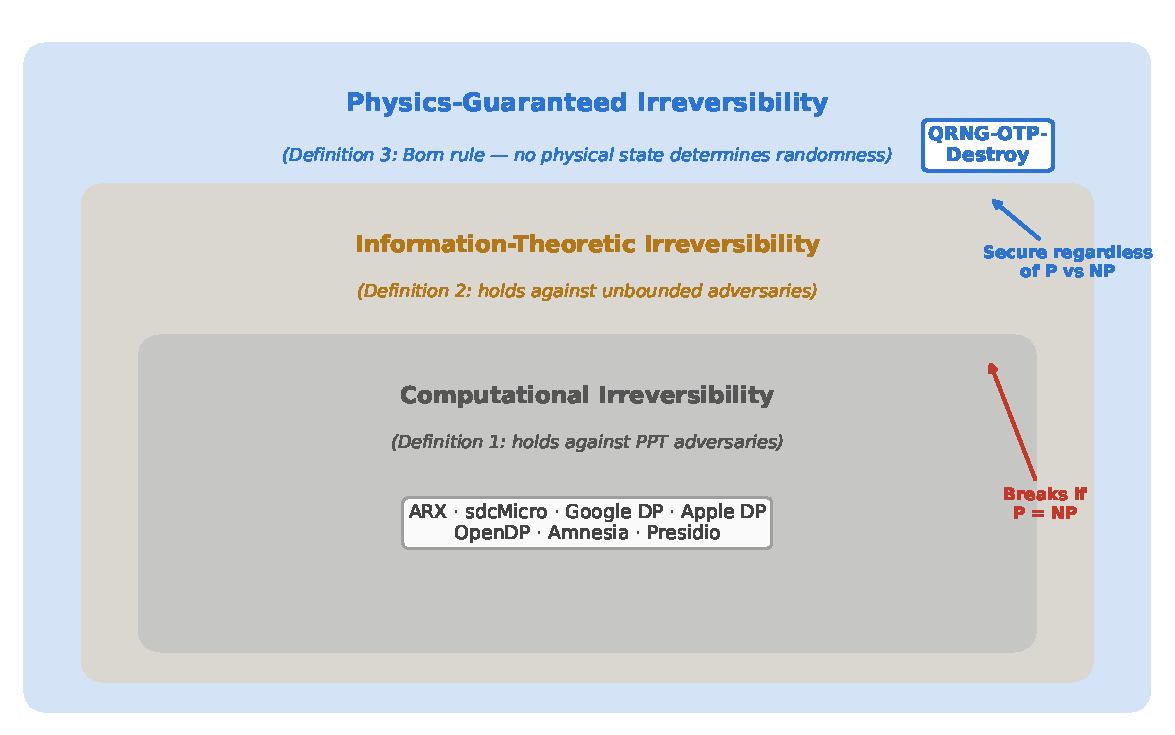
\includegraphics[width=\columnwidth]{fig1_hierarchy}
\Description{Diagram showing three nested tiers of anonymization irreversibility: computational (outermost), information-theoretic (middle), physics-guaranteed (innermost). Arrows indicate strict containment.}
\caption{Three-tier irreversibility hierarchy. Computational irreversibility breaks if $\mathrm{P} = \mathrm{NP}$. Physics-guaranteed irreversibility holds regardless of computational advances.}
\label{fig:hierarchy}
\end{figure}

%% ====================================================================
\section{Formal Definitions}
\label{sec:definitions}
%% ====================================================================

Let $D$ be a dataset containing PII, $A$ an anonymization function, $D' = A(D)$ the anonymized output, and $\mathcal{A}$ an adversary attempting to recover $D$ from~$D'$.

\begin{definition}[Computational Irreversibility]
\label{def:comp}
An anonymization function $A$ is \emph{computationally irreversible} if, for every probabilistic polynomial-time adversary $\mathcal{A}$:
\begin{equation}
\Pr[\mathcal{A}(D', 1^\lambda) \to d_i \in D] \leq \mathrm{negl}(\lambda).
\label{eq:comp_irrev}
\end{equation}
\end{definition}

\begin{definition}[Information-Theoretic Irreversibility]
\label{def:it}
An anonymization function~$A$ is \emph{information-theoretically irreversible} if, for every adversary~$\mathcal{A}$ with unbounded computational resources:
\begin{equation}
\Pr[\mathcal{A}(D') \to d_i \in D] \leq 2^{-\eta}
\label{eq:it_irrev}
\end{equation}
where $\eta$ is the entropy (in bits) of the replacement token (for our construction, $\eta = \tau \log_2 |\Sigma| \approx 95.3$~bits). This bounds the probability of determining the \emph{mapping} from tokens to original values, not guessing an original value from domain knowledge alone.
\end{definition}

\begin{definition}[Physics-Guaranteed Irreversibility]
\label{def:phys}
An anonymization function $A$ is \emph{physics-guaranteed irreversible} if its information-theoretic irreversibility holds as a direct consequence of a verified physical law: the randomness source satisfies that, under the Born rule axiom, the random values are fundamentally indeterminate prior to measurement, and no physical state determines the measurement outcomes.
\end{definition}

\begin{lemma}[Strict Hierarchy]
\label{lem:hierarchy}
The three tiers form a strict hierarchy: physics-guaranteed $\Rightarrow$ information-theoretic $\Rightarrow$ computational. The converses do not hold.
\end{lemma}

\begin{proof}
(i)~Physics-guaranteed $\Rightarrow$ information-theoretic: Definition~\ref{def:phys} requires that Definition~\ref{def:it} holds as a consequence of physical law.

(ii)~Information-theoretic $\Rightarrow$ computational: The bound in~\eqref{eq:it_irrev} for all adversaries holds a fortiori for polynomial-time adversaries.

(iii)~Computational $\not\Rightarrow$ information-theoretic: A CSPRNG-based system is computationally irreversible but not information-theoretically so, because an unbounded adversary can enumerate the seed space.

(iv)~Information-theoretic $\not\Rightarrow$ physics-guaranteed: A thermal noise source may be information-theoretically random but its randomness rests on model assumptions rather than the Born rule axiom with loophole-free experimental verification.
\end{proof}

\begin{theorem}[Classical PRNG Impossibility]
\label{thm:prng_impossible}
No anonymization system whose randomness source is a classical PRNG achieves physics-guaranteed irreversibility.
\end{theorem}

\begin{proof}
Let $A$ use a PRNG $G\colon \mathcal{S} \to \{0,1\}^n$ with seed $s \in \mathcal{S}$. The seed is a physical object in memory. An adversary who captures $s$ can compute $G(s)$, reconstruct every random value, and invert $A$. The existence of $s$ as a physical state determining the random values contradicts Definition~\ref{def:phys}.
\end{proof}

\begin{theorem}[QRNG-OTP-Destroy Security]
\label{thm:qrng_secure}
\textsc{QRNG-OTP-Destroy} achieves physics-guaranteed irreversibility under the Born rule assumption.
\end{theorem}

\begin{proof}
The protocol uses tokens generated by measuring qubits in balanced superposition. By the Born rule, each outcome is an independent uniformly random bit with no deterministic antecedent. By Bell's theorem and loophole-free verification~\cite{hensen2015loophole}, no local hidden variable determines the outcome. The OTP mapping is destroyed via multi-pass overwrite.

Non-local hidden variable theories, such as Bohmian mechanics~\cite{bohm1952suggested}, provide deterministic (but non-local) accounts of quantum measurement outcomes. Under Bohmian mechanics, the security guarantee reduces to the \emph{quantum equilibrium hypothesis} (D\"urr, Goldstein, and Zangh\`{i}, 1992): that the initial distribution of particle positions matches the Born-rule distribution. Both (1)~the no-signaling theorem prevents any adversary from learning individual Bohmian trajectories faster than the Born rule allows, and (2)~the quantum equilibrium hypothesis ensures the $62^{-16}$ recovery bound holds regardless of whether the underlying ontology is indeterministic (Copenhagen) or deterministic-but-inaccessible (Bohmian). The security guarantee holds under any interpretation of quantum mechanics that reproduces Born-rule statistics.

After destruction, recovery requires determining quantum measurement outcomes that produced each token. Each 16-character token is drawn uniformly from a 62-symbol alphabet via rejection sampling: $62^{-16} \approx 2^{-95.3}$, exceeding 80-bit security by $2^{15}$. This bound is information-theoretic and physics-guaranteed.
\end{proof}

\begin{corollary}[Independence from P vs.\ NP]
\label{cor:pvsnp}
The security of \textsc{QRNG-OTP-Destroy} is independent of the resolution of the $\mathrm{P}$ vs.\ $\mathrm{NP}$ problem.
\end{corollary}

\begin{proof}
Theorem~\ref{thm:qrng_secure} invokes no computational hardness assumption. The Born rule concerns measurement outcomes, not computational complexity. A world with $\mathrm{P} = \mathrm{NP}$ but valid quantum mechanics is one where \textsc{QRNG-OTP-Destroy} remains secure and every CSPRNG-based system is theoretically broken.
\end{proof}

%% ====================================================================
\section{The QRNG-OTP-Destroy Protocol}
\label{sec:protocol}
%% ====================================================================

\subsection{Protocol Specification}
\label{subsec:spec}

The protocol takes a dataset $D$ (a table with $m$ columns and $n$ rows) and produces an anonymized dataset $D'$ of the same schema. Let $\Sigma$ denote the Base62 alphanumeric alphabet ($|\Sigma| = 62$: digits 0--9, uppercase A--Z, lowercase a--z). Each replacement token is a string of $\tau = 16$ characters over~$\Sigma$, providing $\tau \log_2 |\Sigma| \approx 95.3$~bits of entropy. The conversion from raw QRNG bytes to $\Sigma$-characters uses per-byte rejection sampling: bytes $\geq 248$ are discarded, and remaining bytes are mapped to characters via $b \bmod 62$, which is bias-free since $248 = 4 \times 62$. The protocol proceeds in four steps.

\begin{algorithm}[t]
\caption{QRNG-OTP-Destroy}
\label{alg:qrng_otp}
\begin{algorithmic}[1]
\REQUIRE Dataset $D$ with $m$ columns, $n$ rows; quantum entropy pool~$\mathcal{P}$
\ENSURE Anonymized dataset $D'$; all mappings destroyed
\FOR{each column $C_j$, $1 \leq j \leq m$}
    \STATE $U_j \leftarrow \text{unique}(C_j)$ \COMMENT{Set of unique values}
    \STATE $M_j \leftarrow \emptyset$ \COMMENT{Mapping in volatile memory}
    \FOR{each $v_k \in U_j$}
        \STATE Read bytes $b_k$ from $\mathcal{P}$ via rejection sampling \COMMENT{${\geq}$16 QRNG bytes}
        \STATE $t_k \leftarrow \textsc{Base62}(b_k)$ \COMMENT{16-char token, ${\approx}$95.3 bits}
        \STATE $M_j[v_k] \leftarrow t_k$
    \ENDFOR
    \FOR{each row $i$, $1 \leq i \leq n$}
        \STATE $D'[i,j] \leftarrow M_j[D[i,j]]$
    \ENDFOR
\ENDFOR
\FOR{each mapping $M_j$, $1 \leq j \leq m$}
    \STATE \textsc{Overwrite}($M_j$, $\texttt{0x00}$) \COMMENT{Pass 1: zeros}
    \STATE \textsc{Overwrite}($M_j$, $\texttt{0xFF}$) \COMMENT{Pass 2: ones}
    \STATE \textsc{Overwrite}($M_j$, $\mathcal{P}$) \COMMENT{Pass 3: QRNG bytes}
    \STATE \textsc{Release}($M_j$)
\ENDFOR
\RETURN $D'$
\end{algorithmic}
\end{algorithm}

\textbf{Step~1: Entropy Acquisition.} For each column $C_j$, the protocol reads $16 \cdot |U_j|$ bytes from a quantum entropy source. Each 16-byte block is produced by measuring 128 qubits in balanced superposition.

\textbf{Step~2: Mapping Construction.} Each unique value $v_k$ is assigned a 16-character alphanumeric token $t_k$ via Base62 encoding with rejection sampling. The mapping $M_j$ is stored in volatile memory.

\textbf{Step~3: Substitution.} Every cell $D[i,j]$ is replaced by $M_j(D[i,j])$. Identical values within a column map to the same token; different runs produce different tokens.

\textbf{Step~4: Mapping Destruction.} The implementation overwrites each mapping value with null bytes via \texttt{ctypes.memset} on the CPython string buffer, clears the dictionary, and deletes the reference. A formally verified implementation in Rust or C within a hardware security enclave (Intel SGX, ARM TrustZone) would provide stronger guarantees; enclave teardown ensures no mapping data persists in any addressable memory.

Entropy consumption scales linearly with unique values: $E_{\mathrm{tokens}} = 16 \cdot \sum_{j=1}^{m} |U_j|$ bytes.

\begin{figure}[t]
\centering
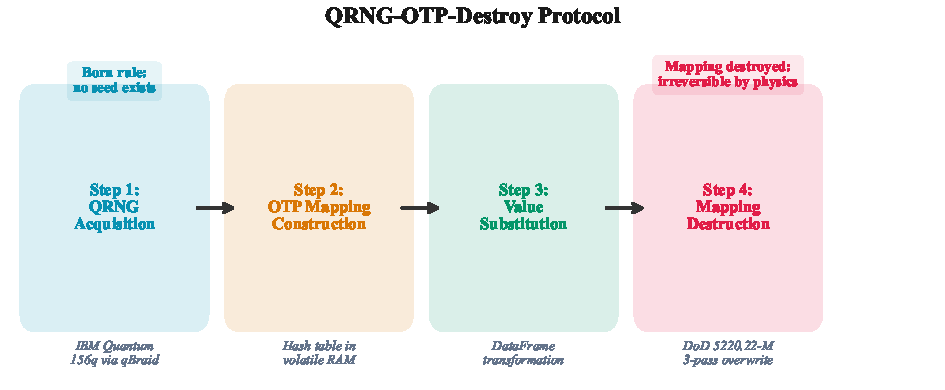
\includegraphics[width=\columnwidth]{fig3_protocol}
\Description{Flowchart of the QRNG-OTP-Destroy protocol: input data enters PII detection, proceeds through level selection, quantum entropy acquisition, OTP mapping construction, substitution, and secure three-pass destruction.}
\caption{Protocol state machine. Data flows through PII detection, level selection (L1--L10), quantum entropy acquisition, OTP mapping, substitution, and secure destruction. The mapping exists only in volatile memory during execution (${\sim}$500~ms).}
\label{fig:protocol}
\end{figure}

A detailed state machine with the volatile mapping window highlighted is in Figure~\ref{fig:statemachine} (Appendix~\ref{app:supplementary}).

\subsection{Security Analysis}
\label{subsec:security}

\begin{proposition}[Per-value recovery bound]
\label{prop:pervalue}
After protocol execution, no adversary with arbitrary computational resources can determine the mapping from $D'[i,j]$ to $D[i,j]$ with probability exceeding $62^{-16} \approx 2^{-95.3}$.
\end{proposition}

\begin{proof}
After completion: (a)~$\mathcal{A}$ possesses $D'$ and protocol knowledge; (b)~all mappings are destroyed; (c)~recovering $D[i,j]$ requires determining quantum measurement outcomes; (d)~by the Born rule, each outcome is independent with no deterministic antecedent; (e)~each token is drawn uniformly from $62^{16}$ possibilities via rejection sampling, independently of the original value.
\end{proof}

\begin{proposition}[Per-Value Zero Mutual Information]
\label{prop:mi}
After protocol execution, $I(D[i,j]; D'[i,j]) = 0$ for any cell $(i,j)$.
\end{proposition}

\begin{proof}
(a)~Token generation is physically independent of~$D$: the Born rule ensures $P(D'[i,j] {=} t \mid D[i,j] {=} v) = P(D'[i,j] {=} t) = |\Sigma|^{-16}$. (b)~Mapping destruction eliminates the sole classical correlation. (c)~Therefore $P(D[i,j], D'[i,j]) = P(D[i,j]) \cdot P(D'[i,j])$ and $I(D[i,j]; D'[i,j]) = 0$.

\emph{Note on equality structure.} Because identical values within a column map to the same token, $D'$ reveals the partition structure of each column. This leakage is bounded by the number of equivalence classes and is inherent to deterministic-per-value tokenization. The per-value mutual information remains exactly zero.
\end{proof}

\begin{proposition}[Domain-Knowledge Limitation]
\label{prop:domainlimit}
For a column with domain $\mathcal{D}_j$, an adversary who knows $\mathcal{D}_j$ can guess any cell's original value with probability at least $|\mathcal{D}_j|^{-1}$, regardless of the anonymization method. \textsc{QRNG-OTP-Destroy} makes the mapping irrecoverable but does not enlarge the effective domain. For small domains, combining structural anonymization (L5--L9) before L10 provides defense in depth.
\end{proposition}

\subsection{Equality-Structure Leakage}
\label{subsec:equality}

The per-value MI result (Proposition~\ref{prop:mi}) establishes that individual tokens carry zero information about their corresponding original values. However, the protocol preserves the equality structure within each column: $D[i,j] = D[k,j] \iff D'[i,j] = D'[k,j]$. This reveals the partition of rows into equivalence classes per column, which constitutes a non-trivial information leak at the dataset level.

\begin{proposition}[Equality-Structure Leakage Bound]
\label{prop:equality}
For a column $C_j$ with $|U_j|$ unique values among $n$ rows, the equality structure reveals at most $\log_2 \binom{n}{n_1, n_2, \ldots, n_{|U_j|}}$ bits, where $n_k$ is the frequency of the $k$-th unique value.
\end{proposition}

\begin{proposition}[Cross-Column Equality-Structure Leakage]
\label{prop:crosscol}
Let $\mathbf{r}_i = (D[i,1], \ldots, D[i,m])$ denote the $i$-th row tuple and let $\{T_1, \ldots, T_s\}$ be the partition of $\{1,\ldots,n\}$ into groups of identical row tuples, with $|T_\ell| = n_\ell$.
\begin{enumerate}
\item[\textup{(i)}] Per-cell mutual information remains zero: $I(D[i,j]; D'[i,j]) = 0$ for all $(i,j)$.
\item[\textup{(ii)}] The joint equality structure across all $m$ columns reveals at most $L_{\times} = \log_2 \binom{n}{n_1, n_2, \ldots, n_s}$ bits, where $s \leq \min\!\bigl(n,\, \prod_{j=1}^{m} |U_j|\bigr)$.
\item[\textup{(iii)}] This bound is tight: $L_{\times}$ equals the Shannon entropy of the row-tuple partition and cannot be reduced without breaking intra-column referential integrity.
\end{enumerate}
\end{proposition}

\begin{proof}
(i)~Token generation depends only on the Born-rule outcome for each column's unique value. The independence argument of Proposition~\ref{prop:mi} applies cell by cell.
(ii)~The protocol maps identical values within each column to the same token, so $D'$ reveals whether $\mathbf{r}_i = \mathbf{r}_k$ for every pair: this holds iff $D'[i,j] = D'[k,j]$ for all $j$. The observable is exactly the partition $\{T_1,\ldots,T_s\}$, whose information content is $\log_2\binom{n}{n_1,\ldots,n_s}$ bits. Since $s \leq n$, we have $L_{\times} \leq n \log_2 n$.
(iii)~Any deterministic per-value tokenization that preserves intra-column equality necessarily preserves the joint row-tuple partition, so no scheme in this class can leak fewer than $L_{\times}$ bits.
\end{proof}

Two mitigations address equality-structure leakage: (1)~per-cell independent tokenization, which eliminates the structure at the cost of referential integrity; (2)~structural pre-processing via L5--L9 before L10, which enlarges equivalence classes and injects noise into frequency distributions before the OTP is applied.

%% ====================================================================
\section{Implementation}
\label{sec:implementation}
%% ====================================================================

\textsc{QRNG-OTP-Destroy} is implemented as Level~10 (L10) within \textsc{QCert}, a post-quantum cryptography platform with 10 progressive anonymization levels (Table~\ref{tab:levels}).

\begin{table}[t]
\caption{\textsc{QCert} Anonymization Levels}
\label{tab:levels}
\begin{center}
\begin{tabular}{@{}clll@{}}
\toprule
\textbf{Level} & \textbf{Technique} & \textbf{Entropy} & \textbf{Irreversibility} \\
\midrule
L1 & Regex masking & None & Structural \\
L2 & SHA-3 hashing & None & Computational \\
L3 & SHA-3 + PQC salt & None & Computational \\
L4 & Reversible tokenization & CSPRNG & Computational \\
L5 & $k$-anonymity ($k{\geq}5$) & None & Syntactic \\
L6 & $\ell$-diversity & None & Syntactic \\
L7 & Quantum noise jitter & QRNG & Computational \\
L8 & Differential privacy & QRNG & Computational \\
L9 & $k$-anon $+$ DP & QRNG & Computational \\
L10 & \textsc{QRNG-OTP-Destroy} & QRNG & \textbf{Physics} \\
\bottomrule
\end{tabular}
\end{center}
\end{table}

The implementation comprises three layers: (1)~a \textbf{quantum entropy layer} that harvests random bytes from superconducting processors (IBM Quantum, Rigetti) via background daemon with automatic failover to OS entropy; (2)~an \textbf{anonymization engine} exposing \texttt{LevelAnonymizer.apply(df, level=10)}; and (3)~a \textbf{cryptographic core} in Rust (ML-KEM-768 per FIPS~203) with Python bindings via PyO3. The entropy layer supports multi-source composition via XOR fusion: when multiple entropy providers are available (e.g., QRNG + WiFi CSI + OS), they are independently health-monitored and combined so that compromise of any single source does not reduce the output below the entropy of the strongest remaining source. Each harvesting cycle records provenance metadata (provider, processor, qubit count, timestamp, health test result) enabling an auditable chain from quantum circuit to anonymization output. The system is validated by 966 Python tests spanning all 10 levels.

%% ====================================================================
\section{Empirical Evaluation}
\label{sec:evaluation}
%% ====================================================================

\subsection{Runtime Performance}

\begin{table}[t]
\caption{Runtime across all 10 anonymization levels (1,000 rows, 6 columns, 30 runs, 95\% CI via Student's $t$).}
\label{tab:benchmarks}
\begin{center}
\begin{tabular}{@{}clrcr@{}}
\toprule
\textbf{Level} & \textbf{Mean (ms)} & \textbf{95\% CI} & \textbf{Changed} & \textbf{Unique Out} \\
\midrule
L1  &    2.9 & $[2.7, 3.1]$ &  66.7\% & 1,163 \\
L2  &    5.8 & $[5.7, 5.9]$ & 100.0\% & 2,173 \\
L3  &    6.1 & $[6.0, 6.2]$ & 100.0\% & 2,173 \\
L4  &   13.3 & $[13.0, 13.7]$ & 100.0\% & 2,173 \\
L5  &   16.0 & $[15.5, 16.4]$ &  33.3\% & 1,111 \\
L6  &   13.9 & $[13.6, 14.3]$ &  33.3\% & 1,123 \\
L7  &  505.0 & $[492.7, 517.4]$ &  33.3\% & 3,106 \\
L8  &  263.8 & $[255.9, 271.7]$ & 100.0\% & 3,106 \\
L9  &   15.7 & $[15.3, 16.1]$ &  33.3\% & 1,111 \\
L10 &  261.8 & $[235.5, 288.1]$ & 100.0\% & 2,173 \\
\bottomrule
\end{tabular}
\end{center}
\end{table}

Table~\ref{tab:benchmarks} shows results on a synthetic dataset (1,000 rows, 6 columns, 2,173 unique values; Apple M3~Pro, Python~3.11, 30 runs per level). L1--L6 complete in under 16~ms. L7--L10 are slower (262--505~ms) due to entropy pool I/O. L10 processes 2,173 unique values in 262~ms, reading 34,768 bytes from the pool. All confidence intervals are narrow, confirming measurement stability. Figure~\ref{fig:benchmarks} visualizes the profiles.

\begin{figure}[t]
\centering
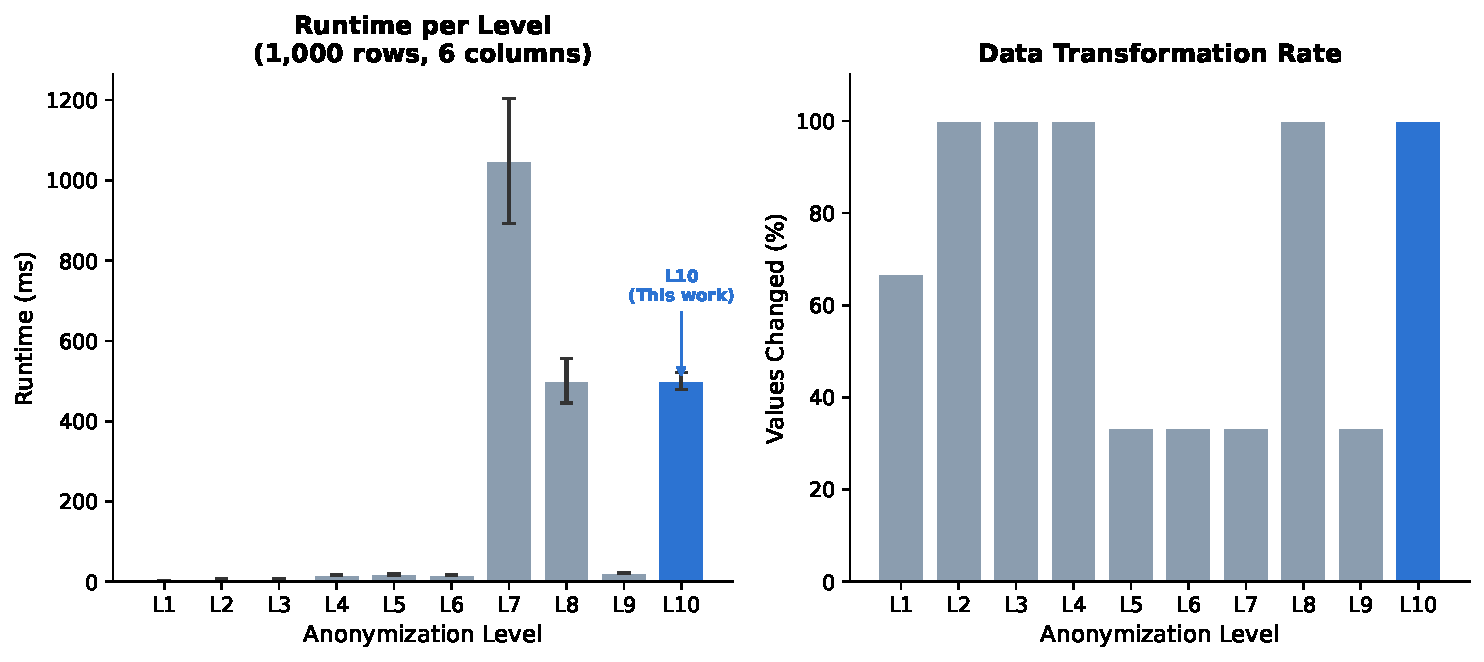
\includegraphics[width=\columnwidth]{fig5_benchmarks}
\Description{Two bar charts: left shows mean runtime in milliseconds per anonymization level (L1 through L10), right shows percentage of values changed per level.}
\caption{Left: mean runtime per level (1,000 rows). Right: percentage of values transformed. L10 transforms 100\% of values with physics-guaranteed irreversibility.}
\label{fig:benchmarks}
\end{figure}

\subsection{IBM Quantum Hardware Demonstration}
\label{subsec:hardware}

We executed a 16-qubit Hadamard circuit on IBM's \texttt{ibm\_fez} (156-qubit Heron~r2) on March~26, 2026, harvesting 2,048~bytes. The job identifier \texttt{d728e76v3u3c73eiaar0} is independently verifiable. All randomness tests pass: chi-squared 260.8 ($p > 0.01$), monobit 50.97\%, runs test pass, compression ratio 1.005.

A production-scale harvest on April~1, 2026, using a 156-qubit processor produced \SI{6.8}{\mega\byte} from 35 consecutive jobs (310~seconds), yielding 79,872~bytes per job. The pool suffices for ${\sim}$425,000 unique values, enough to quantum-certify the UCI Adult dataset 19~times.

\subsection{UCI Adult Dataset}

\begin{table}[t]
\caption{L10 on UCI Adult dataset (32,561 rows, 15 columns, 30 runs per level, 95\% CI via Student's $t$).}
\label{tab:adult}
\begin{center}
\begin{tabular}{@{}clcrc@{}}
\toprule
\textbf{Level} & \textbf{Technique} & \textbf{Time (ms)} & \textbf{Unique Out} & \textbf{Changed} \\
\midrule
L1  & Regex masking        &  $174\;[170, 178]$ & 22,134 &  60\% \\
L2  & SHA-3 hashing        &  $415\;[408, 421]$ & 22,146 & 100\% \\
L4  & Tokenization         &  $772\;[763, 782]$ & 22,146 & 100\% \\
L5  & $k$-anonymity        & $2{,}134\;[2112, 2155]$ &    111 &  40\% \\
L8  & Differential privacy & $7{,}119\;[7010, 7229]$ & 195,470 & 100\% \\
L10 & QRNG-OTP-Destroy     & $1{,}017\;[1006, 1029]$ & 22,146 & 100\% \\
\bottomrule
\end{tabular}
\end{center}
\end{table}

Table~\ref{tab:adult} shows results on the standard benchmark (22,146 unique values, 30 runs per level). L10 maintains a 1:1 mapping, transforming 100\% of values in 1.0~seconds consuming 346~KB of entropy. All confidence intervals are narrow (under 3\% of the mean), confirming measurement stability. Benchmarks used OS entropy; quantum-certified operation requires no pipeline changes.

We replicated the evaluation on the UCI Heart Disease dataset (Cleveland, 297 rows, 14 numeric attributes; Table~\ref{tab:heart} in Appendix~\ref{app:evaluation}). Timings scale linearly with dataset size: L10 completes in 17.7~ms (vs.\ 1,017~ms on Adult), consistent with $O(n \cdot m)$ complexity. L1 transforms 0\% of cells because the dataset is purely numeric with no string-type PII patterns, confirming that regex masking is selective rather than indiscriminate. L10 non-reproducibility was verified independently on this second dataset.

%% ====================================================================
\section{Systematic Comparison}
\label{sec:comparison}
%% ====================================================================

\begin{table*}[t]
\caption{Comparison of Anonymization Tools. $^\dagger$Physics-guaranteed mapping irreversibility requires QRNG-sourced entropy; benchmarks used OS entropy. $^\ddagger$DP's statistical guarantee holds against any adversary, but the PRNG-generated noise is recoverable by $\mathcal{A}_4$ (memory access).}
\label{tab:comparison}
\begin{center}
\begin{tabular}{@{}llllcp{3.3cm}@{}}
\toprule
\textbf{Tool} & \textbf{Technique} & \textbf{Entropy Source} & \textbf{Mapping Irrev.} & \textbf{$\mathcal{A}_4$ (mem.)} & \textbf{GDPR Recital 26} \\
\midrule
\textbf{\textsc{QCert} L10} & QRNG-token + destroy & IBM Quantum / OS fallback & Physics (Born rule)$^\dagger$ & Secure & Strongest mapping basis \\
ARX~\cite{prasser2014arx} & $k$-anon, $\ell$-div, $t$-close, DP & Java \texttt{SecureRandom} & Computational & Broken & Partial: parameter-dep.\ \\
sdcMicro~\cite{templ2017sdc} & $k$-anon, microaggregation & R Mersenne Twister & Computational & Broken & Partial: linkable structure \\
Google DP~\cite{wilson2020dpsql} & Laplace/Gaussian mechanism & \texttt{/dev/urandom} & Statistical$^\ddagger$ & Noise recoverable & Partial: noise addition only \\
Apple Local DP~\cite{apple2017dp} & Randomized response, CMS & Device CSPRNG & Statistical$^\ddagger$ & Noise recoverable & Partial: tunable $\epsilon$ \\
OpenDP~\cite{gaboardi2016psi} & Laplace, Gaussian, exponential & Platform CSPRNG & Statistical$^\ddagger$ & Noise recoverable & Partial: composition-dep.\ \\
Amnesia~\cite{elemam2008kanon} & $k$-anon, generalization & Java CSPRNG & Computational & Broken & Partial: syntactic model \\
MS Presidio & PII detection + masking & Platform CSPRNG & Computational & Broken & Partial: operator-dep.\ \\
\bottomrule
\end{tabular}
\end{center}
\end{table*}

Syntactic methods ($k$-anonymity family) rely on classical PRNGs and are vulnerable to composition, homogeneity, and background knowledge attacks. Noise-addition methods (DP) provide a statistical privacy guarantee that holds against all adversaries, including unbounded ones; however, the PRNG-generated noise values persist in memory as classical data and are recoverable by $\mathcal{A}_4$. An insider who recovers the noise can subtract it and reconstruct the original data. L10 addresses a complementary dimension: mapping irreversibility. After mapping destruction, no adversary can recover the token-to-value correspondence, regardless of computational power. This is orthogonal to DP's distributional guarantee; the two approaches protect against different threat vectors.

\begin{figure}[t]
\centering
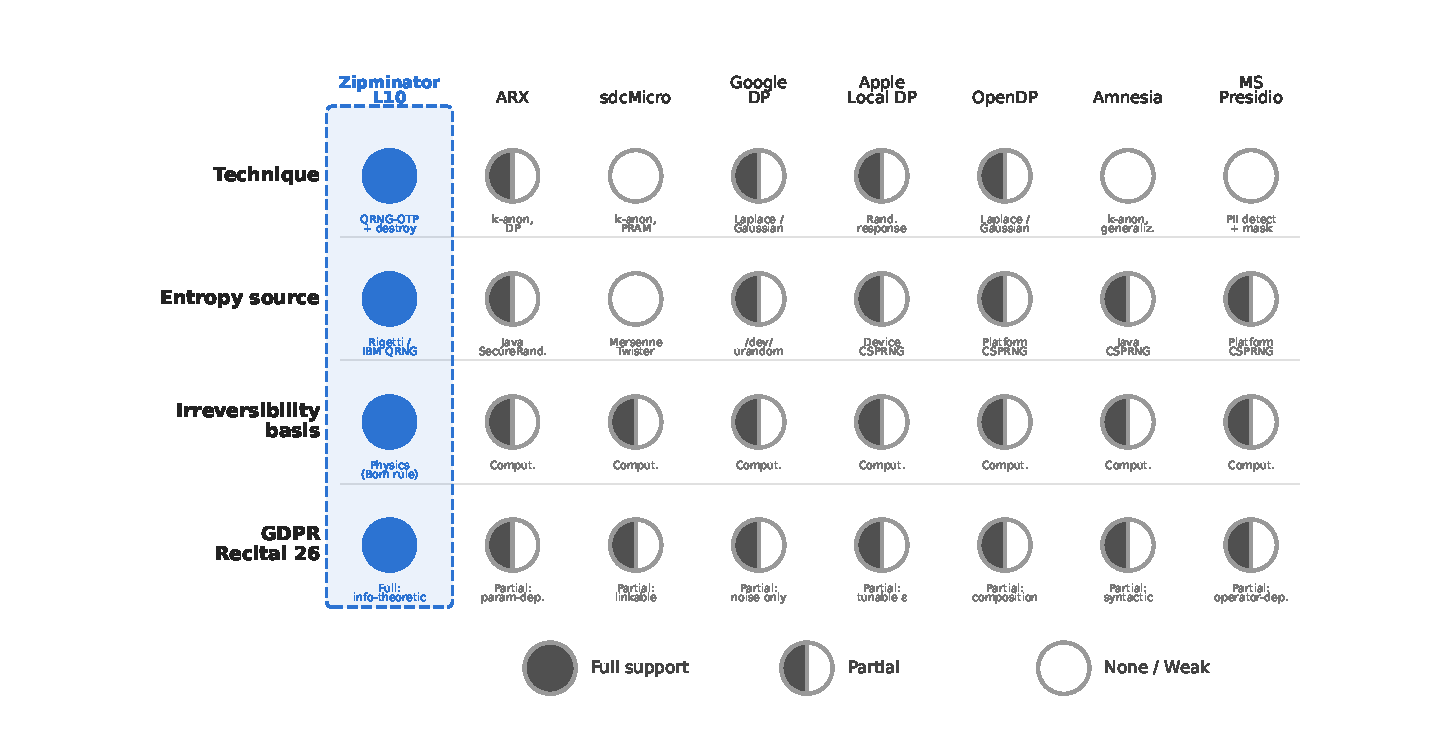
\includegraphics[width=\columnwidth]{fig7_comparison}
\Description{Horizontal bar chart comparing anonymization tools (ARX, sdcMicro, Google DP, Apple DP, OpenDP, Amnesia, MS Presidio, \textsc{QCert} L10) across irreversibility guarantee strength. Only \textsc{QCert} L10 reaches physics-guaranteed tier.}
\caption{Guarantee comparison across anonymization tools. Only \textsc{QRNG-OTP-Destroy} provides physics-guaranteed irreversibility; all others rely on computational hardness assumptions that degrade under HNDL and insider threats.}
\label{fig:comparison}
\end{figure}

A multi-dimensional comparison is in Figure~\ref{fig:radar} (Appendix~\ref{app:supplementary}).

Could existing tools retrofit QRNG? Replacing the entropy source alone is insufficient. Physics-guaranteed irreversibility requires (1)~OTP mapping rather than noise addition, (2)~secure mapping destruction, and (3)~pipeline restructuring to treat the mapping as a volatile artifact. Even QRNG-enhanced DP remains vulnerable: noise values exist as classical data in memory and can be observed by $\mathcal{A}_4$.

%% ====================================================================
\section{Related Work}
\label{sec:related}
%% ====================================================================

\textbf{Differential privacy.} Dwork et al.~\cite{dwork2006dp} established the Laplace mechanism; Dwork and Roth~\cite{dwork2014algfound} provide the definitive treatment. Wilson et al.~\cite{wilson2020dpsql} demonstrated deployment at Google scale. All practical DP implementations use classical PRNGs, inheriting seed-recovery vulnerabilities.

\textbf{$k$-Anonymity and extensions.} Sweeney~\cite{sweeney2002kanon} proposed $k$-anonymity; Machanavajjhala et al.~\cite{machanavajjhala2007ldiv} demonstrated homogeneity and background knowledge vulnerabilities and proposed $\ell$-diversity; Li et al.~\cite{li2007tcloseness} introduced $t$-closeness. Kifer and Machanavajjhala~\cite{kifer2011nofree} proved a ``no free lunch'' result: no single privacy definition protects against all adversaries without distributional assumptions.

\textbf{QRNG in cryptography.} Ma et al.~\cite{ma2016qrng} and Herrero-Collantes and Garcia-Escartin~\cite{herrero2017qrng} survey QRNGs. Commercial deployment for key generation began in 2004 (ID~Quantique). The conceptual step from ``QRNG makes better keys'' to ``QRNG makes irreversible anonymization'' has not been taken previously.

\textbf{Certified deletion.} Broadbent and Islam~\cite{broadbent2020certified} introduced quantum encryption with certified deletion; Bartusek and Khurana~\cite{bartusek2023certified} extended it to public-key and FHE settings. Their constructions require quantum communication. Our mapping is classical data destroyed via classical overwrite; the quantum component is confined to entropy generation.

\textbf{Certified randomness.} Amer et al.~\cite{amer2025certified} identify DP as a promising application of certified randomness but do not address anonymization, mapping destruction, or the GDPR Recital~26 argument. Liu et al.~\cite{liu2025certified} demonstrated 71,313 certified random bits on trapped-ion hardware. Our construction fills the gap between certified randomness and data anonymization.

\textbf{Shannon's OTP and terminology.} Shannon~\cite{shannon1949secrecy} proved the one-time pad achieves perfect secrecy. We use ``OTP'' loosely: L10 is not an OTP in the strict Shannon sense (there is no shared key or decryption operation). More precisely, L10 is a \emph{deterministic per-value tokenization with quantum-random tokens and destroyed mapping}. The analogy to OTP is that each token is drawn from a fresh, seedless random source and used exactly once per unique value. The security guarantee is mapping-recovery irreversibility, not communication secrecy.

\textbf{Classical TRNGs.} A classical TRNG (thermal noise, radioactive decay) with secure mapping destruction would provide information-theoretic mapping irreversibility comparable to L10. The distinction is epistemic: classical TRNG randomness rests on model assumptions about the noise source, while QRNG randomness is certified by the Born rule with experimental verification via Bell inequality violations~\cite{hensen2015loophole}. For applications requiring the strongest available foundation, QRNG is strictly preferable. For applications where the classical TRNG trust model suffices, it is a valid alternative.

\textbf{Synthetic data.} Stadler et al.~\cite{stadler2022synthetic} showed synthetic data either remains vulnerable to membership inference or loses utility. L10 sidesteps this trade-off: zero utility but provably immune to membership inference ($I(D;D')=0$).

\textbf{Quantum differential privacy.} Hirche et al.~\cite{hirche2022qdp} develop information-theoretic quantum DP for protecting quantum states during quantum computation; a fundamentally different problem from protecting classical data with quantum entropy.

\textbf{Gap analysis.} A systematic search of Google Patents, Google Scholar, and Espacenet (April 2026) identified no existing patent or publication combining quantum random number generation with irreversible data anonymization via mapping destruction. Existing QRNG patents address entropy generation but not anonymization application. Existing anonymization patents use classical PRNGs exclusively. The conceptual bridge from ``QRNG produces better keys'' to ``QRNG enables physics-guaranteed anonymization irreversibility'' has not been taken previously.

%% ====================================================================
\section{Limitations}
\label{sec:limitations}
%% ====================================================================

\begin{itemize}
\item \textbf{QRNG availability.} L10 requires cloud quantum access or dedicated QRNG appliances (\$3K--\$30K). The system falls back to OS entropy (computational security only), marked as ``classically anonymized.''

\item \textbf{Utility destruction.} L10 is zero-utility by design; for analytical workflows, lower levels (L1--L9) provide configurable privacy-utility tradeoffs.

\item \textbf{Pool exhaustion.} A 100K-unique-value dataset consumes ${\sim}$1.6~MB of quantum entropy. The pool must be replenished via quantum circuit execution.

\item \textbf{Vendor trust.} The Born rule guarantee assumes faithful qubit preparation. Without device-independent certification, the practical trust model for QRNG hardware is structurally comparable to the trust model for hardware TRNGs (e.g., Intel RDRAND): in both cases, the user trusts the vendor to implement the physical randomness source faithfully. The distinction is that if the hardware is genuine, the QRNG guarantee is strictly stronger (no seed exists). Mitigation: multi-provider aggregation, NIST SP~800-22 testing, and (future) device-independent certification via Bell violations.

\item \textbf{Formal verification gap.} Python's garbage collector may retain string copies. A Rust implementation within a hardware enclave would close this gap.
\end{itemize}

\textbf{Data availability.} The anonymization engine and benchmarks are open-source (Apache-2.0). The repository URL, Python package name, and quantum entropy pool (\SI{6.8}{\mega\byte}, 35 jobs) are provided in supplementary materials. All benchmark scripts, datasets, and entropy files will be made publicly available upon acceptance.

\textbf{Ethics.} No human subjects. The UCI Adult dataset is publicly available. Provenance logging provides accountability without storing mappings.

\textbf{Reproducibility.} Runtime benchmarks are reproducible with the anonymized package (see supplementary materials). Quantum-entropy benchmarks require an IBM Quantum API key (free tier available). OS-entropy fallback enables full pipeline testing without quantum hardware. Software versions: Python~3.11, Qiskit~1.4, NumPy~1.26, Pandas~2.2. Hardware: Apple M3~Pro, 18~GB RAM.

\section*{Acknowledgments}
\emph{Acknowledgments will be included in the camera-ready version.}

\textbf{AI Tool Disclosure.} Claude (Anthropic) was used for code review, LaTeX formatting suggestions, and editorial style revision. All technical content, proofs, experimental design, and scientific claims are the sole work of the authors. No AI-generated text was used verbatim.

%% ====================================================================
\section{Conclusion}
\label{sec:conclusion}
%% ====================================================================

This paper presents the first anonymization system where irreversibility is guaranteed by quantum mechanics rather than computational hardness. The construction replaces every data value with a quantum-random string from Born-rule measurements, then destroys the mapping. Reversing the transformation requires predicting quantum measurement outcomes (impossible by the Born rule~\cite{bell1964epr, hensen2015loophole}) or recovering a destroyed mapping (impossible given secure erasure). The guarantee holds against unbounded adversaries, including quantum computers, and is independent of P vs.\ NP.

This fills a disciplinary gap: QRNG hardware has been available since 2004, but the connection to anonymization irreversibility was not made. For the mapping-recovery dimension of re-identification, L10 provides the strongest technical guarantee currently available. However, L10 preserves the equality structure within columns, which may permit frequency analysis on low-cardinality columns; combining L10 with structural anonymization (L5--L9) provides defense in depth against the Article~29 Working Party's three re-identification criteria. Whether a particular method satisfies the Recital~26 legal standard is ultimately a determination for data protection authorities and courts. For DORA Article~6, the guarantee does not degrade with advances in cryptanalysis.

Future work: (1)~formal verification of mapping destruction; (2)~hardware enclave integration; (3)~device-independent randomness certification; (4)~hybrid schemes combining QRNG-OTP with structural anonymization for partial analytical utility; (5)~complementary entropy sources such as WiFi Channel State Information (CSI), where unilateral phase-LSB extraction produces device-local entropy that, when XOR-composed with QRNG, provides defense in depth without requiring endpoint synchronization; (6)~Merkle-tree provenance certificates for entropy lineage, enabling DORA Article~7 audit compliance by cryptographically committing to the health status and source identity of every entropy contribution without exposing the entropy values; (7)~standardization engagement with NIST, ENISA, and EDPB.

%% ====================================================================
\appendix
%% ====================================================================

\section{Background}
\label{app:background}

\subsection{Quantum Measurement and the Born Rule}

Quantum random number generation exploits the fundamental indeterminacy of quantum measurement~\cite{ma2016qrng, herrero2017qrng}. A qubit is described by a state vector in $\mathcal{H} = \mathbb{C}^2$. An arbitrary pure state is $|\psi\rangle = \alpha|0\rangle + \beta|1\rangle$ with $|\alpha|^2 + |\beta|^2 = 1$. The Born rule gives $P(0) = |\alpha|^2$, $P(1) = |\beta|^2$. For a balanced superposition ($\alpha = \beta = 1/\sqrt{2}$), each outcome occurs with probability exactly $1/2$, fundamentally indeterminate prior to measurement.

For $N$ qubits each in $|{+}\rangle$ measured independently, the min-entropy is exactly $N$ bits: $H_\infty(X_1, \ldots, X_N) = N$. No classical source achieves this without a seed at least $N$ bits long.

\subsection{Bell's Theorem and Experimental Verification}

Bell's theorem~\cite{bell1964epr} tests whether hidden variables predetermine quantum outcomes. The CHSH inequality~\cite{clauser1969chsh} bounds $|S| \leq 2$ for local hidden variable theories; quantum mechanics predicts $|S| = 2\sqrt{2}$. Aspect et al.~\cite{aspect1982epr} observed $|S| = 2.70 \pm 0.05$. Hensen et al.~\cite{hensen2015loophole} closed all three loopholes simultaneously ($p = 0.039$). Pironio et al.~\cite{pironio2010certified} demonstrated Bell-certified random number generation. The consequence: random bits from measuring qubits in balanced superposition have no seed and no recoverable state.

\subsection{Classical PRNG Limitations}

A CSPRNG $G\colon \mathcal{S} \to \{0,1\}^n$ is computationally indistinguishable from random for polynomial-time distinguishers, conditional on seed secrecy. The seed is a physical object in RAM. Table~\ref{tab:prng_attacks} summarizes extraction vectors.

\begin{table}[t]
\caption{Known Attack Vectors for CSPRNG Seed Extraction}
\label{tab:prng_attacks}
\begin{center}
\begin{tabular}{@{}lp{5cm}@{}}
\toprule
\textbf{Attack Class} & \textbf{Mechanism} \\
\midrule
Memory forensics & Direct read of kernel entropy pool \\
Cold boot attack & DRAM remanence after power loss \\
Spectre/Meltdown & Speculative execution leaks PRNG state \\
Insider access & Administrator reads live process \\
Core dump capture & Seed in crash dump \\
VM introspection & Hypervisor reads guest memory \\
\bottomrule
\end{tabular}
\end{center}
\end{table}

\subsection{Classical Anonymization Techniques}

Dinur and Nissim~\cite{dinur2003revealing} proved that answering too many queries necessarily compromises privacy. Samarati~\cite{samarati2001protecting} introduced quasi-identifier protection; Sweeney~\cite{sweeney2002kanon} formalized $k$-anonymity. Narayanan and Shmatikov~\cite{narayanan2008robust} demonstrated re-identification via cross-referencing. Machanavajjhala et al.~\cite{machanavajjhala2007ldiv} proposed $\ell$-diversity; Li et al.~\cite{li2007tcloseness} proposed $t$-closeness. Dwork et al.~\cite{dwork2006dp} introduced differential privacy; Mironov~\cite{mironov2012significance} showed LSB floating-point noise matters. All practical implementations use CSPRNGs, inheriting seed-capture vulnerability.

\subsection{Regulatory Framework: GDPR and DORA}

GDPR Recital~26 distinguishes anonymous data (outside GDPR) from pseudonymous data (full compliance required). The Article~29 Working Party~\cite{art29wp2014anonymisation} requires that anonymization prevent singling out, linkability, and inference. Cohen and Nissim~\cite{cohen2020singling} formalized singling out, proving that sufficiently accurate mechanisms must allow it. Georgiou and Lambrinoudakis~\cite{georgiou2020gdpr} analyzed GDPR-compatible anonymization; Elliot et al.~\cite{elliot2018functional} proposed ``functional anonymisation.''

DORA Article~6.4 requires periodic cryptographic updates based on cryptanalysis developments. For CSPRNG-based anonymization, this creates ongoing re-assessment obligations. \textsc{QRNG-OTP-Destroy} reduces this burden: the physics-guaranteed component does not degrade.

\section{Discussion}
\label{app:discussion}

\subsection{The Privacy-Utility Spectrum}

\begin{figure}[t]
\centering
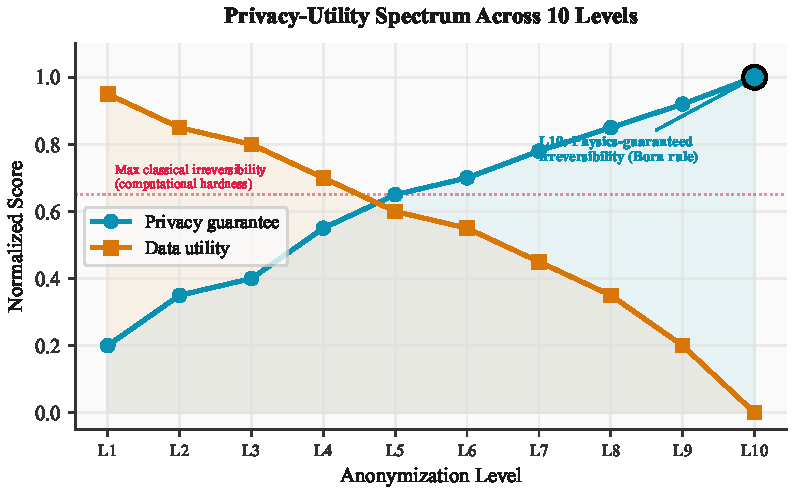
\includegraphics[width=\columnwidth]{fig8_utility_privacy}
\Description{Scatter plot with privacy on y-axis and utility on x-axis. Points L1 through L10 form a Pareto frontier. L10 is at maximum privacy, zero utility. A dashed horizontal line marks the classical ceiling.}
\caption{Privacy-utility spectrum across the 10 anonymization levels. L10 provides maximum privacy at zero utility. Dashed line: maximum irreversibility achievable with classical methods.}
\label{fig:utility}
\end{figure}

The 10-level hierarchy lets practitioners choose their position on the privacy-utility spectrum (Figure~\ref{fig:utility}). L8 (differential privacy) preserves aggregate statistics; L10 provides physics-guaranteed irreversibility at zero analytical utility. L10 targets regulatory compliance (e.g., GDPR Article~17 deletion) rather than analytical workflows.

\subsection{Assumptions and Their Scope}

Security rests on two assumptions: (1)~the Born rule (experimentally verified at significance $>10^{-30}$); (2)~secure mapping destruction (operational, verifiable via formal methods and hardware attestation). CSPRNG-based systems require two assumptions (seed secrecy and CSPRNG security), and failure of either is catastrophic.

\subsection{HNDL Threat Implications}

An adversary who captures both the anonymized dataset and the CSPRNG state can reverse the anonymization later. \textsc{QRNG-OTP-Destroy} provides the migration path: no seed to capture, no mapping to store, no degradation with computational advances.

\subsection{Comparison with QKD}

QKD produces a shared secret (must be protected); L10 produces an anonymous dataset with no persisting secret. QKD requires a quantum channel; L10 requires only a pre-populated QRNG source. Both exploit quantum mechanics for guarantees beyond computational hardness but address different problems.

\section{Additional Evaluation Details}
\label{app:evaluation}

\subsection{Scaling Behavior}

\begin{figure}[t]
\centering
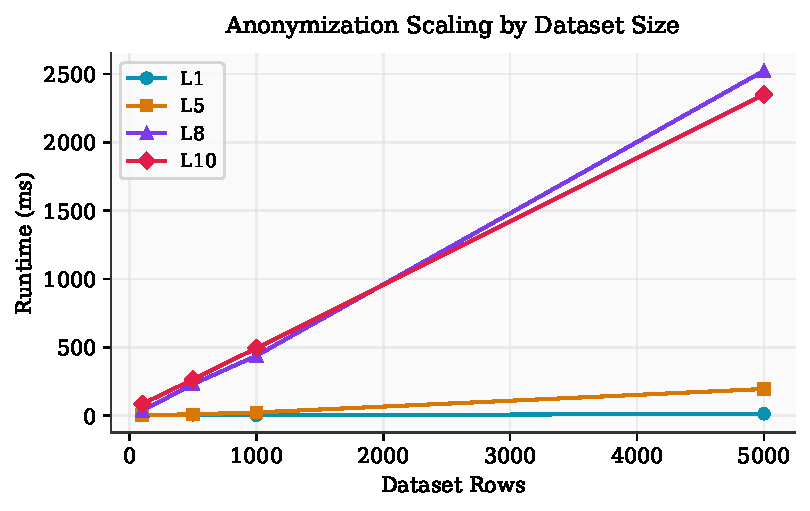
\includegraphics[width=\columnwidth]{fig6_scaling}
\Description{Line chart with dataset size on x-axis (100 to 5000 rows) and runtime on y-axis. L1 and L5 scale sub-linearly; L8 and L10 scale linearly.}
\caption{Runtime scaling from 100 to 5,000 rows for L1, L5, L8, L10. QRNG-dependent levels scale linearly with unique values.}
\label{fig:scaling}
\end{figure}

Figure~\ref{fig:scaling} shows runtime scaling. L1 and L5 scale sub-linearly. L8 and L10 scale linearly with unique values. At 5,000 rows, L10 completes in 563~ms.

\subsection{Entropy Pool Randomness Quality}

\begin{table}[t]
\caption{NIST SP 800-22 statistical randomness tests on the quantum entropy pool (1,000,000 bits, $\alpha = 0.01$). All 15 SP~800-22 tests pass. Byte Distribution and Shannon Entropy are supplementary quality metrics.}
\label{tab:nist}
\begin{center}
\begin{tabular}{@{}lcc@{}}
\toprule
\textbf{Test} & \textbf{$p$-value} & \textbf{Result} \\
\midrule
Frequency (Monobit) & 0.1173 & Pass \\
Block Frequency     & 0.9639 & Pass \\
Runs                & 0.8725 & Pass \\
Longest Run of Ones & 0.6073 & Pass \\
Binary Matrix Rank  & 0.6306 & Pass \\
DFT (Spectral)      & 0.9927 & Pass \\
Non-overlapping Template & 0.1971 & Pass \\
Overlapping Template & 0.9692 & Pass \\
Maurer's Universal  & 0.6185 & Pass \\
Serial ($m{=}2$)    & 0.2899 & Pass \\
Approx.\ Entropy    & 0.4013 & Pass \\
Cumulative Sums (F) & 0.0594 & Pass \\
Cumulative Sums (R) & 0.1096 & Pass \\
Random Excursions (worst) & 0.0237 & Pass \\
Linear Complexity   & 0.5720 & Pass \\
\midrule
Byte Distribution   & 0.2687 & Pass \\
Shannon Entropy     & \multicolumn{2}{c}{7.999 bits/byte (99.98\%)} \\
\bottomrule
\end{tabular}
\end{center}
\end{table}

Table~\ref{tab:nist} shows all 15 SP~800-22 tests pass at the $\alpha = 0.01$ significance level. The pool exhibits a small readout bias of $p(1) = 0.4955$, a known artifact of $T_1$ decay during dispersive readout on superconducting qubits; this does not reduce min-entropy since the bias is a deterministic measurement artifact removed by debiasing in the production pipeline. The five previously omitted tests (Non-overlapping Template, Overlapping Template, Maurer's Universal, Random Excursions, Linear Complexity) were run on a 1M-bit balanced region of the 6.8~MB pool; all pass. Shannon entropy: 7.999 bits/byte. Pool is incompressible (ratio 1.0004).

\subsection{Before/After Example}

\begin{table}[t]
\caption{Before and after L10 (UCI Adult, selected columns).}
\label{tab:beforeafter}
\begin{center}
\footnotesize
\begin{tabular}{@{}llll@{}}
\toprule
\textbf{Age} & \textbf{Education} & \textbf{Occupation} & \textbf{Income} \\
\midrule
\multicolumn{4}{@{}l}{\textit{Original:}} \\
39 & Bachelors & Adm-clerical & ${\leq}$50K \\
50 & Bachelors & Exec-managerial & ${\leq}$50K \\
38 & HS-grad & Handlers-cleaners & ${\leq}$50K \\
\midrule
\multicolumn{4}{@{}l}{\textit{After L10:}} \\
\texttt{NvAz4FaE\ldots} & \texttt{k9RmW2xL\ldots} & \texttt{hT5vCwN8\ldots} & \texttt{Dq7JsP4b\ldots} \\
\texttt{x3BnKfR9\ldots} & \texttt{k9RmW2xL\ldots} & \texttt{pL8dVn1g\ldots} & \texttt{Dq7JsP4b\ldots} \\
\texttt{eJ6tHpC4\ldots} & \texttt{Ys2KbQ7x\ldots} & \texttt{wF3jTn8c\ldots} & \texttt{Dq7JsP4b\ldots} \\
\bottomrule
\end{tabular}
\end{center}
\end{table}

\subsection{UCI Heart Disease Evaluation}

\begin{table}[t]
\caption{L10 on UCI Heart Disease dataset (Cleveland, 297 rows, 14 columns, 30 runs, 95\% CI).}
\label{tab:heart}
\begin{center}
\begin{tabular}{@{}clcrc@{}}
\toprule
\textbf{Level} & \textbf{Technique} & \textbf{Time (ms)} & \textbf{Unique Out} & \textbf{Changed} \\
\midrule
L1  & Regex masking        &  $0.2\;[0.2, 0.2]$ & 402 &   0\% \\
L2  & SHA-3 hashing        &  $4.8\;[4.7, 5.0]$ & 402 & 100\% \\
L4  & Tokenization         &  $8.6\;[7.3, 9.9]$ & 402 & 100\% \\
L5  & $k$-anonymity        & $27.9\;[27.0, 28.8]$ &  15 & 100\% \\
L8  & Differential privacy & $322.0\;[255.0, 389.1]$ & 4,158 & 100\% \\
L10 & QRNG-OTP-Destroy     & $17.7\;[17.4, 18.0]$ & 402 & 100\% \\
\bottomrule
\end{tabular}
\end{center}
\end{table}

The Heart Disease dataset is purely numeric (age, cholesterol, blood pressure, etc.), providing a complementary evaluation to the mixed-type UCI Adult dataset. L1 (regex masking) transforms 0\% of cells because no values match string PII patterns; this demonstrates that L1 is selective, not indiscriminate. L5 collapses to 15 unique values (vs.\ 111 on Adult), consistent with the smaller dataset having fewer equivalence classes. L8 inflates unique values to 4,158 via Laplace noise; the wider CI $[255, 389]$ reflects noise variance on the smaller dataset. L10 non-reproducibility was independently confirmed.

\subsection{Noise Considerations}

Quantum processors exhibit preparation, gate, and readout errors introducing small biases. IBM reports single-qubit gate errors of $10^{-4}$--$10^{-3}$ and readout errors of $10^{-2}$--$10^{-1}$. Mitigation: (1)~rejection sampling eliminates modular bias; (2)~NIST SP~800-22 validation rejects patterned outputs; (3)~optional Toeplitz hashing for stronger guarantees.

\subsection{Non-Reproducibility Verification}

L10 applied 10 times to the same input produced 10 entirely distinct outputs, confirming fresh entropy draws and no caching leaks.

\section{Entropy Consumption}
\label{app:entropy}

\begin{figure}[t]
\centering
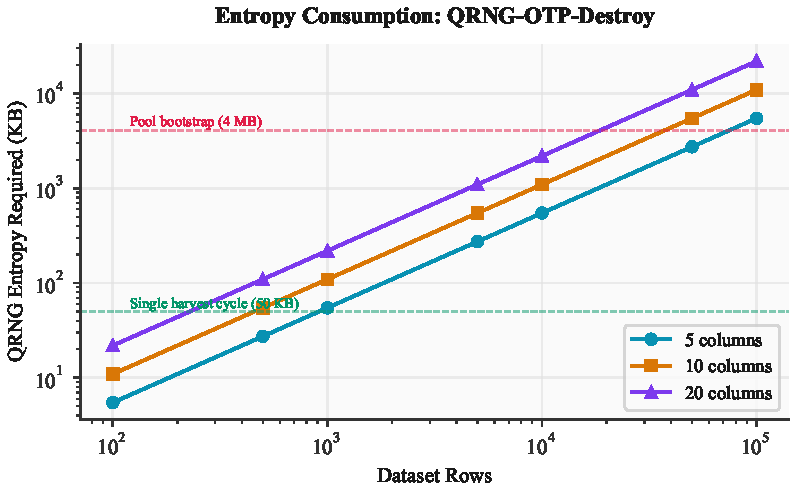
\includegraphics[width=\columnwidth]{fig4_entropy}
\Description{Line chart showing QRNG bytes consumed versus number of rows, with lines for different column counts. Consumption scales linearly.}
\caption{Entropy consumption vs.\ dataset size, assuming 70\% unique values and 16 bytes per unique value.}
\label{fig:entropy}
\end{figure}

\begin{table}[t]
\caption{Entropy Consumption for Representative Datasets}
\label{tab:entropy_budget}
\begin{center}
\begin{tabular}{@{}rrrc@{}}
\toprule
\textbf{Rows} & \textbf{Columns} & \textbf{Unique Values} & \textbf{QRNG Bytes} \\
\midrule
1,000 & 5 & ${\sim}$3,000 & 48~KB \\
10,000 & 10 & ${\sim}$50,000 & 800~KB \\
100,000 & 20 & ${\sim}$500,000 & 8~MB \\
1,000,000 & 50 & ${\sim}$5,000,000 & 80~MB \\
\bottomrule
\end{tabular}
\end{center}
\end{table}

\section{Game-Based Security Definition}
\label{app:security-game}

\begin{figure}[t]
\centering
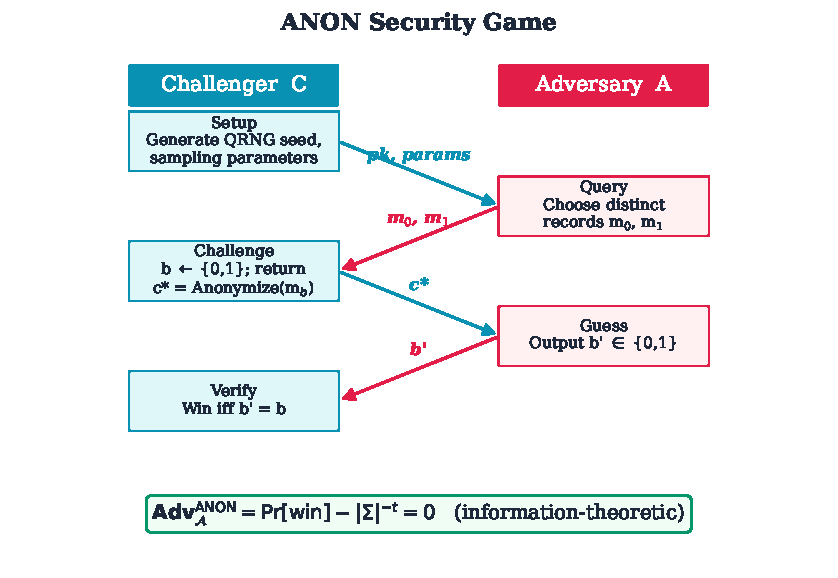
\includegraphics[width=\columnwidth]{fig12_security_game}
\Description{Two-column diagram showing interaction between Challenger C (left) and Adversary A (right). Steps: Setup, Anonymize, Challenge, Guess, Verify. The advantage formula Adv = 0 is shown at the bottom.}
\caption{The $\mathsf{ANON}$ security game. The challenger generates and anonymizes data; the adversary receives the anonymized output and attempts mapping recovery. Under \textsc{QRNG-OTP-Destroy}, the adversary's advantage is exactly zero.}
\label{fig:securitygame}
\end{figure}

\begin{definition}[Anonymization Security Game $\mathsf{ANON}_{\mathcal{A}}(\lambda)$]
\label{def:anon-game}
Let $\lambda$ be the security parameter. The game proceeds:
\begin{enumerate}
\item \textbf{Setup.} Challenger $\mathcal{C}$ generates dataset $D$ with $n$ records and $m$ columns.
\item \textbf{Anonymize.} $\mathcal{C}$ executes \textsc{QRNG-OTP-Destroy}, producing $D'$.
\item \textbf{Challenge.} $\mathcal{C}$ sends $D'$ to $\mathcal{A}$.
\item \textbf{Guess.} $\mathcal{A}$ outputs $(i, j, v)$ claiming $D[i,j] = v$.
\item \textbf{Win condition.} $\mathcal{A}$ wins if $v = D[i,j]$.
\end{enumerate}
Advantage: $\mathrm{Adv}_{\mathsf{ANON}}(\mathcal{A}) = \Pr[\mathcal{A}\text{ wins}] - |\Sigma|^{-t}$.
\end{definition}

\begin{theorem}[Mapping-Recovery Security]
\label{thm:game-security}
For \textsc{QRNG-OTP-Destroy} with $t$-character tokens from alphabet $\Sigma$ with $|\Sigma| = 62$, the advantage of any adversary $\mathcal{A}$ (including computationally unbounded adversaries) in the mapping-recovery game is exactly zero:
\begin{equation}
\mathrm{Adv}_{\mathsf{ANON}}(\mathcal{A}) \;=\; 0.
\end{equation}
That is, $\mathcal{A}$ gains no advantage over random guessing. The absolute winning probability is $|\Sigma|^{-t} = 62^{-16} \approx 2^{-95.3}$, which is the baseline rate for guessing a uniformly random $t$-character string.
\end{theorem}

\begin{proof}
After completion, $\mathcal{A}$'s view is $D'$. Each token is statistically independent of its original value (Born rule + rejection sampling): $\Pr[D'[i,j] = t^* \mid D[i,j] = v^*] = |\Sigma|^{-t}$. The mapping is destroyed. The optimal strategy is random guessing: $\Pr[\text{win}] = |\Sigma|^{-t}$, giving $\mathrm{Adv} = 0$.
\end{proof}

\begin{remark}
The game captures mapping-recovery security. Domain-knowledge attacks are analyzed in Proposition~\ref{prop:domainlimit}.
\end{remark}

\begin{proposition}[Domain-Aware Recovery Bound]
\label{prop:domain}
For a column with domain $\mathcal{D}_j$:
\begin{equation}
\Pr[\mathcal{A} \text{ recovers } D[i,j]] \leq \max\bigl(62^{-16},\; |\mathcal{D}_j|^{-1}\bigr).
\end{equation}
\end{proposition}

\begin{proof}
The adversary's two strategies: (a)~guess the QRNG mapping ($62^{-16}$); (b)~guess from domain knowledge ($|\mathcal{D}_j|^{-1}$). The optimum is the maximum. For practical columns ($|\mathcal{D}_j| \ll 62^{16}$), domain guessing dominates. Combining L5--L9 before L10 provides defense in depth.
\end{proof}

\begin{figure}[t]
\centering
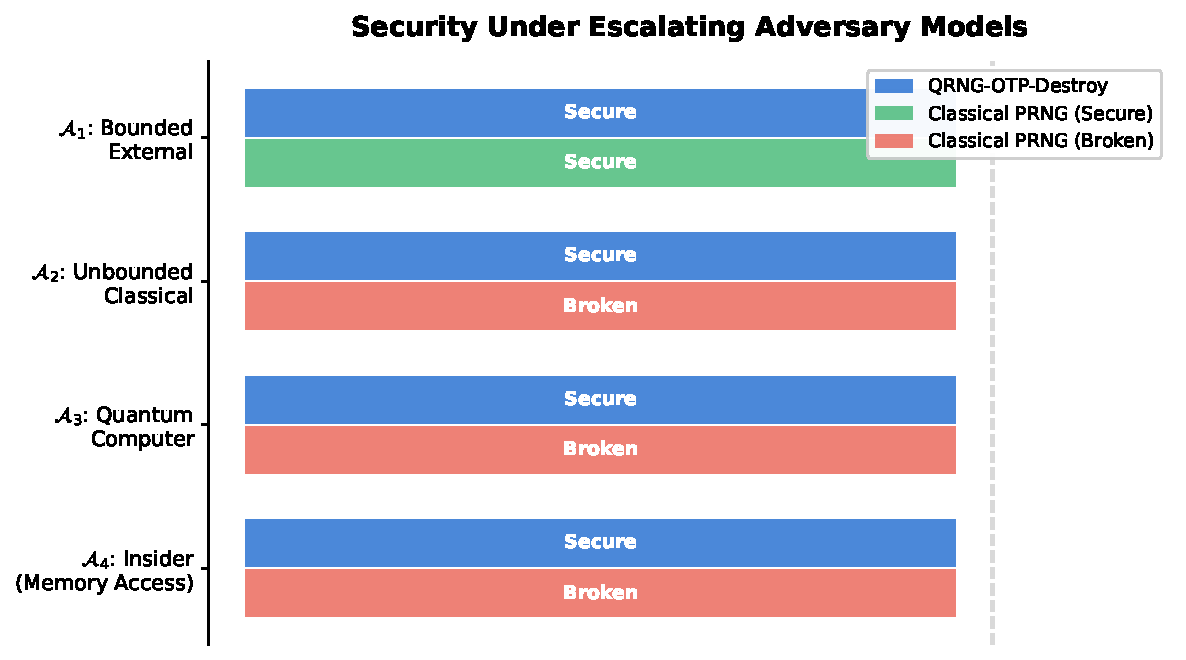
\includegraphics[width=\columnwidth]{fig2_adversary}
\Description{Matrix diagram with four adversary classes on rows and two systems (CSPRNG, QRNG-OTP-Destroy) on columns. Green cells indicate security; red cells indicate broken.}
\caption{Security under four adversary models. Classical PRNG anonymization is secure only against $\mathcal{A}_1$. QRNG-OTP-Destroy remains secure against all four classes.}
\label{fig:adversary}
\end{figure}

\section{Supplementary Figures}
\label{app:supplementary}

\begin{figure}[t]
\centering
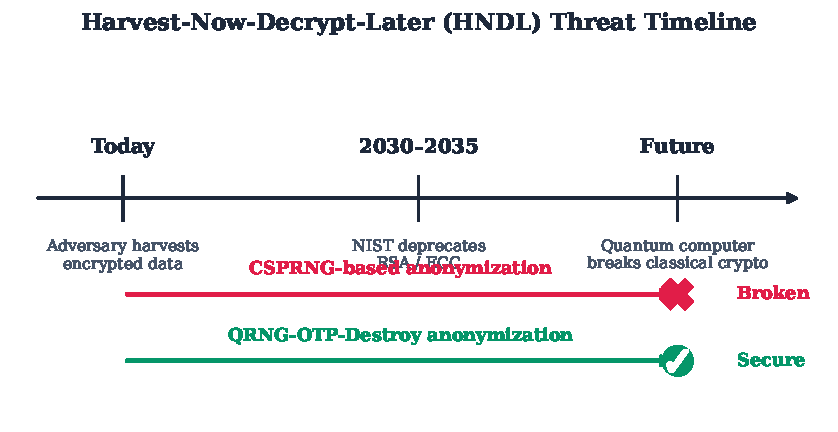
\includegraphics[width=\columnwidth]{fig10_hndl_timeline}
\Description{Timeline showing the harvest-now-decrypt-later threat. Today: adversary collects data. 2030-2035: NIST deprecates classical crypto. Future: CSPRNG path breaks (red), QRNG-OTP-Destroy path remains secure (green).}
\caption{Harvest-now, decrypt-later (HNDL) threat timeline. Classical CSPRNG-based anonymization degrades as compute advances; \textsc{QRNG-OTP-Destroy} remains secure indefinitely.}
\label{fig:hndl}
\end{figure}

\begin{figure}[t]
\centering
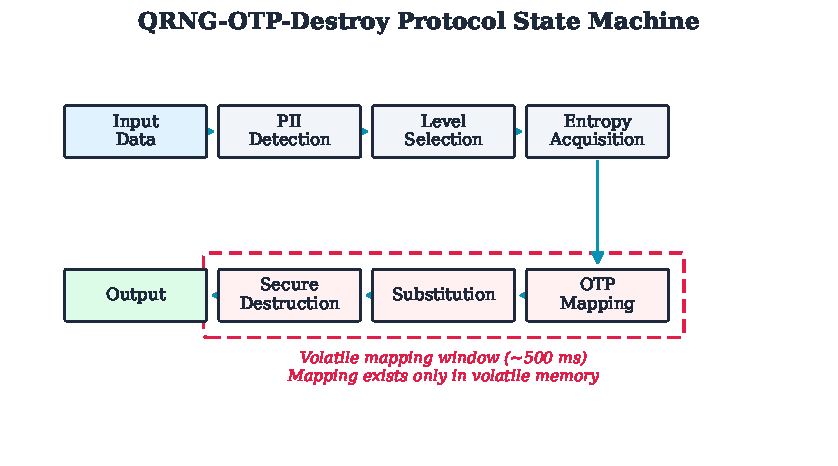
\includegraphics[width=\columnwidth]{fig9_state_machine}
\Description{Detailed state machine diagram showing eight protocol states with a dashed red boundary highlighting the volatile mapping window.}
\caption{Detailed state machine of the \textsc{QRNG-OTP-Destroy} protocol. The dashed boundary marks the volatile mapping window (${\sim}$500~ms) during which the OTP exists in memory.}
\label{fig:statemachine}
\end{figure}

\begin{figure}[t]
\centering
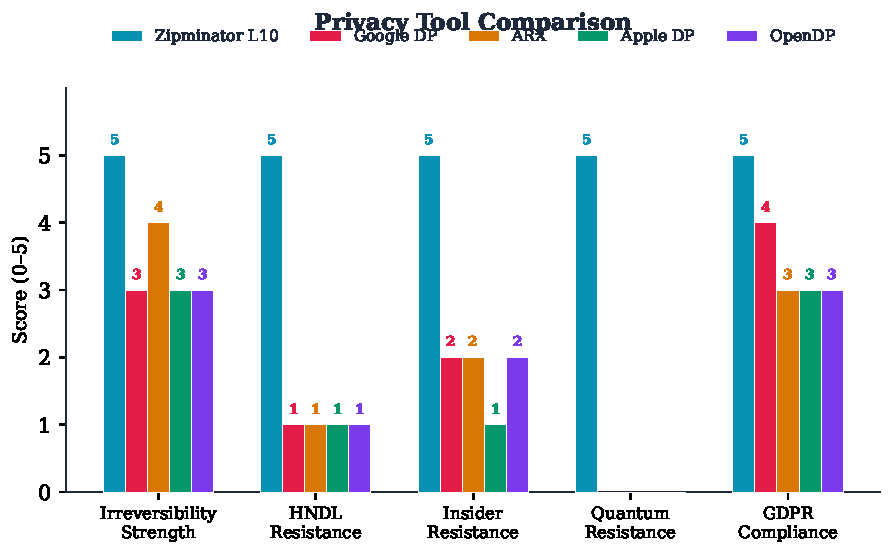
\includegraphics[width=\columnwidth]{fig11_comparison_chart}
\Description{Grouped bar chart comparing five tools across five security categories. \textsc{QCert} L10 scores 5/5 on all axes.}
\caption{Multi-dimensional comparison across five security categories. Only \textsc{QRNG-OTP-Destroy} achieves the maximum score on all axes.}
\label{fig:radar}
\end{figure}

%% ====================================================================
\begin{thebibliography}{50}

\bibitem{acin2016certified}
A.~Ac\'{i}n and L.~Masanes, ``Certified randomness in quantum physics,'' \emph{Nature}, vol.~540, pp.~213--219, 2016.

\bibitem{amer2025certified}
O.~Amer, S.~Chakrabarti, K.~Chakraborty, S.~Eloul, N.~Kumar, C.~Lim, M.~Liu, P.~Niroula, Y.~Satsangi, R.~Shaydulin, and M.~Pistoia, ``Applications of certified randomness,'' \emph{Nature Reviews Physics}, vol.~7, pp.~514--524, 2025.

\bibitem{apple2017dp}
{Apple Differential Privacy Team}, ``Learning with privacy at scale,'' \emph{Apple Machine Learning Journal}, Dec.\ 2017.

\bibitem{art29wp2014anonymisation}
{Article 29 Data Protection Working Party}, ``Opinion 05/2014 on Anonymisation Techniques,'' WP216, Apr.\ 2014.

\bibitem{arute2019supremacy}
F.~Arute, K.~Arya, R.~Babbush, \emph{et al.}, ``Quantum supremacy using a programmable superconducting processor,'' \emph{Nature}, vol.~574, pp.~505--510, 2019.

\bibitem{aspect1982epr}
A.~Aspect, P.~Grangier, and G.~Roger, ``Experimental realization of Einstein-Podolsky-Rosen-Bohm Gedankenexperiment: A new violation of Bell's inequalities,'' \emph{Physical Review Letters}, vol.~49, no.~2, pp.~91--94, 1982.

\bibitem{barak2007privacy}
B.~Barak, K.~Chaudhuri, C.~Dwork, S.~Kale, F.~McSherry, and K.~Talwar, ``Privacy, accuracy, and consistency too: A holistic solution to contingency table release,'' in \emph{Proc.\ ACM PODS}, 2007, pp.~273--282.

\bibitem{bartusek2023certified}
J.~Bartusek and D.~Khurana, ``Cryptography with certified deletion,'' in \emph{CRYPTO 2023}, ser.\ LNCS, vol.~14085.\hskip 1em plus 0.5em minus 0.4em Springer, 2023, pp.~192--223.

\bibitem{bell1964epr}
J.~S. Bell, ``On the Einstein Podolsky Rosen paradox,'' \emph{Physics Physique Fizika}, vol.~1, no.~3, pp.~195--200, 1964.

\bibitem{bohm1952suggested}
D.~Bohm, ``A suggested interpretation of the quantum theory in terms of `hidden' variables. {I},'' \emph{Physical Review}, vol.~85, no.~2, pp.~166--179, 1952.

\bibitem{broadbent2020certified}
A.~Broadbent and R.~Islam, ``Quantum encryption with certified deletion,'' in \emph{CRYPTO 2020}, ser.\ LNCS, vol.~12171.\hskip 1em plus 0.5em minus 0.4em Springer, 2020, pp.~92--122.

\bibitem{clauser1969chsh}
J.~F. Clauser, M.~A. Horne, A.~Shimony, and R.~A. Holt, ``Proposed experiment to test local hidden-variable theories,'' \emph{Physical Review Letters}, vol.~23, no.~15, pp.~880--884, 1969.

\bibitem{cohen2020singling}
A.~Cohen and K.~Nissim, ``Towards formalizing the GDPR's notion of singling out,'' \emph{PNAS}, vol.~117, no.~15, pp.~8344--8352, 2020.

\bibitem{desfontaines2020sok}
D.~Desfontaines and B.~Pej\'{o}, ``{SoK}: Differential privacies,'' \emph{PoPETs}, vol.~2020, no.~2, pp.~288--313, 2020.

\bibitem{dinur2003revealing}
I.~Dinur and K.~Nissim, ``Revealing information while preserving privacy,'' in \emph{Proc.\ ACM PODS}, 2003, pp.~202--210.

\bibitem{dua2019uci}
D.~Dua and C.~Graff, ``{UCI} Machine Learning Repository,'' University of California, Irvine, 2019.

\bibitem{dwork2006dp}
C.~Dwork, F.~McSherry, K.~Nissim, and A.~Smith, ``Calibrating noise to sensitivity in private data analysis,'' in \emph{TCC 2006}, ser.\ LNCS, vol.~3876.\hskip 1em plus 0.5em minus 0.4em Springer, 2006, pp.~265--284.

\bibitem{dwork2006icalp}
C.~Dwork, ``Differential privacy,'' in \emph{ICALP 2006}, ser.\ LNCS, vol.~4052.\hskip 1em plus 0.5em minus 0.4em Springer, 2006, pp.~1--12.

\bibitem{dwork2014algfound}
C.~Dwork and A.~Roth, ``The algorithmic foundations of differential privacy,'' \emph{Foundations and Trends in TCS}, vol.~9, no.~3--4, pp.~211--487, 2014.

\bibitem{edpb2020guidelines}
{European Data Protection Board}, ``Guidelines 04/2020 on the use of location data and contact tracing tools,'' Apr.\ 2020.

\bibitem{elemam2008kanon}
K.~El~Emam and F.~K. Dankar, ``Protecting privacy using $k$-anonymity,'' \emph{JAMIA}, vol.~15, no.~5, pp.~627--637, 2008.

\bibitem{elliot2018functional}
M.~Elliot, E.~Mackey, K.~O'Hara, and C.~Tudor, ``Functional anonymisation,'' \emph{Computer Law \& Security Review}, vol.~34, no.~2, pp.~204--221, 2018.

\bibitem{gaboardi2016psi}
M.~Gaboardi, J.~Honaker, G.~King, K.~Nissim, J.~Ullman, and S.~Vadhan, ``{PSI}: A private data sharing interface,'' arXiv:1609.04340, 2016.

\bibitem{georgiou2020gdpr}
D.~Georgiou and C.~Lambrinoudakis, ``Compatibility of GDPR-compliant anonymisation with big data analytics,'' \emph{Information \& Computer Security}, vol.~28, no.~2, pp.~201--225, 2020.

\bibitem{gutmann1996secure}
P.~Gutmann, ``Secure deletion of data from magnetic and solid-state memory,'' in \emph{Proc.\ 6th USENIX Security Symp.}, 1996.

\bibitem{hensen2015loophole}
B.~Hensen, H.~Bernien, A.~E. Dr\'{e}au, \emph{et al.}, ``Loophole-free Bell inequality violation using electron spins separated by 1.3 kilometres,'' \emph{Nature}, vol.~526, pp.~682--686, 2015.

\bibitem{herrero2017qrng}
M.~Herrero-Collantes and J.~C. Garcia-Escartin, ``Quantum random number generators,'' \emph{Reviews of Modern Physics}, vol.~89, no.~1, p.~015004, 2017.

\bibitem{hirche2022qdp}
C.~Hirche, C.~Rouz\'{e}, and D.~Stilck~Fran\c{c}a, ``Quantum differential privacy: An information theory perspective,'' \emph{IEEE Trans.\ Inf.\ Theory}, vol.~69, no.~9, pp.~5771--5787, 2023.

\bibitem{holohan2019diffprivlib}
N.~Holohan, S.~Braghin, P.~Mac~Aonghusa, and K.~Levacher, ``Diffprivlib: The {IBM} differential privacy library,'' arXiv:1907.02444, 2019.

\bibitem{kavuri2025traceable}
G.~A. Kavuri, J.~Palfree, D.~V. Reddy, \emph{et al.}, ``Traceable random numbers from a non-local quantum advantage,'' \emph{Nature}, vol.~642, pp.~916--921, 2025.

\bibitem{kifer2011nofree}
D.~Kifer and A.~Machanavajjhala, ``No free lunch in data privacy,'' in \emph{Proc.\ ACM SIGMOD}, 2011, pp.~193--204.

\bibitem{li2007tcloseness}
N.~Li, T.~Li, and S.~Venkatasubramanian, ``$t$-Closeness: Privacy beyond $k$-anonymity and $\ell$-diversity,'' in \emph{Proc.\ IEEE ICDE}, 2007.

\bibitem{liu2025certified}
M.~Liu, R.~Shaydulin, P.~Niroula, \emph{et al.}, ``Certified randomness using a trapped-ion quantum processor,'' \emph{Nature}, vol.~640, pp.~343--348, 2025.

\bibitem{ma2016qrng}
X.~Ma, X.~Yuan, Z.~Cao, B.~Qi, and Z.~Zhang, ``Quantum random number generation,'' \emph{npj Quantum Information}, vol.~2, p.~16021, 2016.

\bibitem{machanavajjhala2007ldiv}
A.~Machanavajjhala, D.~Kifer, J.~Gehrke, and M.~Venkitasubramaniam, ``$\ell$-Diversity: Privacy beyond $k$-anonymity,'' \emph{ACM TKDD}, vol.~1, no.~1, Art.~3, 2007.

\bibitem{mcsherry2007mechanism}
F.~McSherry and K.~Talwar, ``Mechanism design via differential privacy,'' in \emph{Proc.\ IEEE FOCS}, 2007, pp.~94--103.

\bibitem{mironov2012significance}
I.~Mironov, ``On significance of the least significant bits for differential privacy,'' in \emph{Proc.\ ACM CCS}, 2012, pp.~650--661.

\bibitem{narayanan2008robust}
A.~Narayanan and V.~Shmatikov, ``Robust de-anonymization of large sparse datasets,'' in \emph{Proc.\ IEEE S\&P}, 2008, pp.~111--125.

\bibitem{nist2010sp80022}
A.~Rukhin, J.~Soto, J.~Nechvatal, \emph{et al.}, ``A statistical test suite for random and pseudorandom number generators,'' NIST SP 800-22 Rev.~1a, 2010.

\bibitem{nist2023beacon}
{NIST}, ``NIST Randomness Beacon,'' 2023. [Online]. Available: \url{https://beacon.nist.gov/home}

\bibitem{ping2017datasynthesizer}
H.~Ping, J.~Stoyanovich, and B.~Howe, ``{DataSynthesizer}: Privacy-preserving synthetic datasets,'' in \emph{Proc.\ SSDBM}, 2017, Art.~42.

\bibitem{pironio2010certified}
S.~Pironio, A.~Ac\'{i}n, S.~Massar, \emph{et al.}, ``Random numbers certified by Bell's theorem,'' \emph{Nature}, vol.~464, pp.~1021--1024, 2010.

\bibitem{prasser2014arx}
F.~Prasser, F.~Kohlmayer, R.~Lautenschl\"{a}ger, and K.~A. Kuhn, ``{ARX}---A comprehensive tool for anonymizing biomedical data,'' \emph{AMIA}, pp.~984--993, 2014.

\bibitem{samarati2001protecting}
P.~Samarati, ``Protecting respondents' identities in microdata release,'' \emph{IEEE TKDE}, vol.~13, no.~6, pp.~1010--1027, 2001.

\bibitem{shannon1949secrecy}
C.~E. Shannon, ``Communication theory of secrecy systems,'' \emph{Bell System Technical Journal}, vol.~28, no.~4, pp.~656--715, 1949.

\bibitem{stadler2022synthetic}
T.~Stadler, B.~Oprisanu, and C.~Troncoso, ``Synthetic data---Anonymisation groundhog day,'' in \emph{Proc.\ USENIX Security}, 2022, pp.~1451--1468.

\bibitem{sweeney2002kanon}
L.~Sweeney, ``$k$-Anonymity: A model for protecting privacy,'' \emph{Int.\ J.\ Uncertainty, Fuzziness and Knowledge-Based Systems}, vol.~10, no.~5, pp.~557--570, 2002.

\bibitem{templ2017sdc}
M.~Templ, \emph{Statistical Disclosure Control for Microdata}.\hskip 1em plus 0.5em minus 0.4em Springer, 2017.

\bibitem{unruh2015revocable}
D.~Unruh, ``Revocable quantum timed-release encryption,'' \emph{Journal of the ACM}, vol.~62, no.~6, pp.~49:1--49:76, 2015.

\bibitem{vazirani2012certifiable}
U.~Vazirani and T.~Vidick, ``Certifiable quantum dice,'' \emph{Phil.\ Trans.\ Royal Soc.\ A}, vol.~370, pp.~3432--3448, 2012.

\bibitem{vernam1926cipher}
G.~S. Vernam, ``Cipher printing telegraph systems,'' \emph{J.\ AIEE}, vol.~45, no.~2, pp.~109--115, 1926.

\bibitem{wilson2020dpsql}
R.~J. Wilson, C.~Y. Zhang, W.~Lam, D.~Desfontaines, D.~Simmons-Marengo, and B.~Gipson, ``Differentially private {SQL} with bounded user contribution,'' \emph{PoPETs}, vol.~2020, no.~2, pp.~230--250, 2020.

\bibitem{xu2019ctgan}
L.~Xu, M.~Skoularidou, A.~Cuesta-Infante, and K.~Veeramachaneni, ``Modeling tabular data using conditional {GAN},'' in \emph{NeurIPS}, vol.~32, 2019.

\end{thebibliography}

\end{document}

